\section{Problem and Data Description}
\label{sec:data}

\subsection{Motivation and Problem Formulation}
\subsubsection{Motivation and Research Objectives}
Recognizing clothing categories from images provides a compact setting for studying how a learning pipeline and its input representation influence classification. This assignment compares architectural families on a common image classification task rather than changing the dataset for each model. Following the course handbook~\cite{handbook}, the intended comparison includes a linear classifier, a multilayer perceptron (MLP), a convolutional neural network (CNN), an LSTM and a Transformer.

The central research question is whether additional nonlinear capacity and image-specific structure improve classification enough to justify their parameter and computational costs. At the source snapshot examined in this draft, the data pipeline and the first three model implementations are available; the sequence models and the final comparative experiments remain incomplete~\cite{code}. Consequently, architectural expectations below are hypotheses, not measured rankings.

\subsubsection{Classification Task: Inputs, Outputs and Prediction Unit}
The prediction unit is one Fashion-MNIST image. Each input has one grayscale channel and spatial dimensions $28\times28$. The target is one integer label in $\{0,\ldots,9\}$. A model returns ten real-valued logits, one per class, and the predicted class is the index of the largest logit. All implemented models retain the same target space and differ in how they represent and process the pixels.

\subsubsection{Mathematical Formulation and Main Challenges}
Let $\mathcal{D}=\{(x_i,y_i)\}_{i=1}^{N}$, with $x_i\in\mathbb{R}^{1\times28\times28}$ and $y_i\in\{0,\ldots,9\}$. A classifier $f_{\theta}$ produces $z_i=f_{\theta}(x_i)\in\mathbb{R}^{10}$. Training minimizes the mean cross-entropy on the training partition, while validation data select the checkpoint. The held-out test set is reserved for evaluating the selected model.

The low image resolution limits fine texture information, and visually similar garment categories can share silhouettes. A flattened representation must learn spatial relationships through its weights, whereas convolution explicitly reuses local filters. These differences motivate examining errors and computational cost alongside aggregate accuracy.

\subsection{Fashion-MNIST Dataset}
\subsubsection{Source, Version, License and Labeling Process}
Fashion-MNIST was introduced by Xiao, Rasul and Vollgraf as a benchmark of fashion-product images~\cite{fashionpaper}. The implementation obtains the official train and test files through \texttt{torchvision.datasets.FashionMNIST}; it does not collect new images or manually relabel the supplied targets~\cite{code}. The upstream project publishes an MIT license~\cite{fashionrepo}. The precise downloaded-file provenance and checksums for the group's experimental cache are \textbf{TBD}.

\subsubsection{Sample Counts, Class Definitions and File Formats}
The benchmark contains 60,000 official training images and 10,000 official test images, with ten categories~\cite{fashionpaper}. Images and labels are distributed in IDX files, with compressed downloads provided by the upstream repository~\cite{fashionrepo}. The image payload alone contains $70{,}000\times28\times28=54{,}880{,}000$ one-byte pixel values; this excludes labels, file headers and compression effects. The project retains the official test partition and creates its validation partition from the official training pool.

Table~\ref{tab:distribution} lists the category names and the counts recorded for the project's 51,000-image training subset. Each image has one class annotation. No additional task or extension dataset is evidenced in the inspected Assignment 1 source and stored outputs.

\subsubsection{Dataset Bias and Limitations}
The benchmark consists of small grayscale product images rather than unrestricted photographs. Performance on it does not establish robustness to real backgrounds, color variation, occlusion, camera changes or categories outside its ten labels. In addition, an approximately balanced class histogram does not imply equal difficulty across classes. These limitations must be considered before generalizing any eventual test result.

\subsection{Exploratory Data Analysis}
\subsubsection{Class Distribution and Imbalance Analysis}
The EDA script uses the saved training indices, so its statistics describe the training subset rather than the entire 60,000-image official training pool. The recorded class counts sum to 51,000. The smallest class contains 5,030 images and the largest contains 5,168, giving
\begin{equation}
 r_{\mathrm{imbalance}}=\frac{\max_c n_c}{\min_c n_c}
 =\frac{5168}{5030}\approx1.0274.
\end{equation}
Thus, the subset is nearly balanced, although its random split is not exactly class-balanced. The current configuration uses neither class reweighting nor resampling. Macro-F1 remains useful because it gives every class equal weight and can expose differences hidden by an aggregate correct-prediction rate.

\begin{table}[htbp]
\centering
\caption{Class counts in the stored training-subset EDA output.}
\label{tab:distribution}
\begin{tabular}{@{}rlr@{}}
\toprule
Label & Class & Training images \\
\midrule
0 & T-shirt/top & 5,030 \\
1 & Trouser & 5,073 \\
2 & Pullover & 5,110 \\
3 & Dress & 5,142 \\
4 & Coat & 5,131 \\
5 & Sandal & 5,108 \\
6 & Shirt & 5,058 \\
7 & Sneaker & 5,168 \\
8 & Bag & 5,115 \\
9 & Ankle boot & 5,065 \\
\midrule
 & Total & 51,000 \\
\bottomrule
\end{tabular}
\end{table}

\begin{figure}[htbp]
\centering
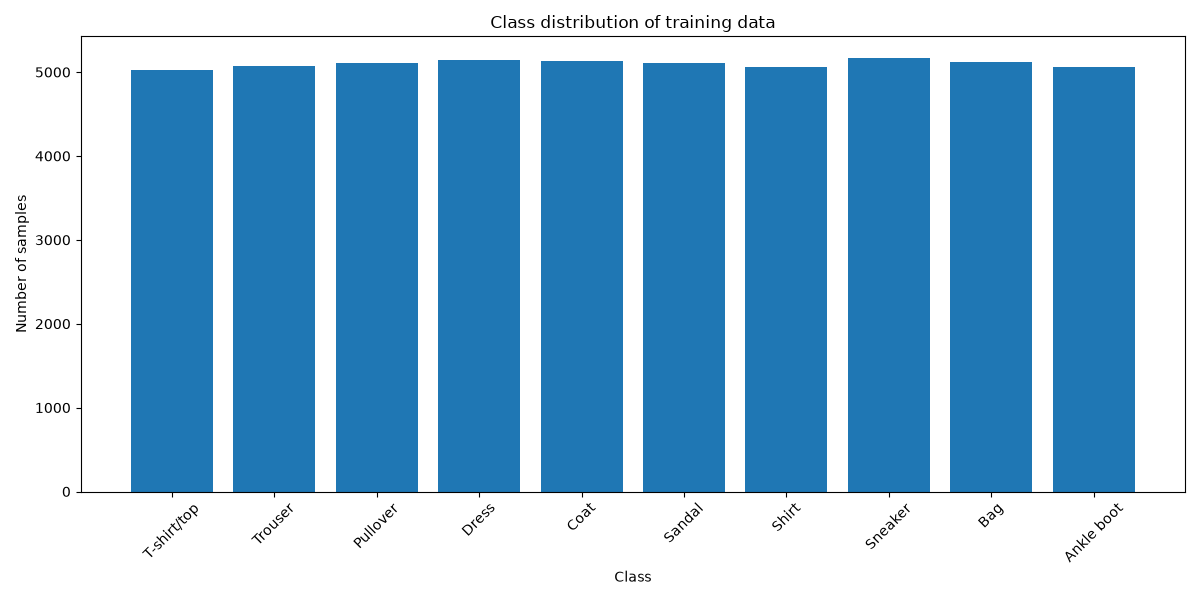
\includegraphics[width=\linewidth]{images/class_distribution.png}
\caption{Training-subset class distribution, reproduced from the EDA artifact stored in the cited source snapshot.}
\label{fig:distribution}
\end{figure}
\FloatBarrier

\subsubsection{Image Dimensions, Channels and Pixel Statistics}
The stored EDA file records raw image dimensions of $28\times28$ and a channel-first model input shape of $1\times28\times28$. After conversion from integer pixels to $[0,1]$, the training-subset minimum and maximum are 0 and 1. The recorded mean is $\mu=0.2856669724$ and the sample standard deviation is $\sigma=0.3528567851$. These values describe scaled pixels \emph{before} standardization, not the final range of normalized inputs.

The implementation computes the statistics over all training-subset pixels and uses the sample standard deviation, with \texttt{unbiased=True}. Validation and test pixels do not participate in estimating these values. Table~\ref{tab:pixelstats} summarizes the stored measurements.

\begin{table}[htbp]
\centering
\caption{Stored training-subset statistics before normalization.}
\label{tab:pixelstats}
\begin{tabular}{@{}lr@{}}
\toprule
Property & Value \\
\midrule
Number of images & 51,000 \\
Input shape & $1\times28\times28$ \\
Scaled pixel range & $[0,1]$ \\
Mean & 0.285667 \\
Sample standard deviation & 0.352857 \\
Class imbalance ratio & 1.027435 \\
\bottomrule
\end{tabular}
\end{table}

\subsubsection{Representative Samples and Visual Ambiguity}
Figure~\ref{fig:samples} contains one training image from each class. The EDA script selects the first available example of each label in the indexed training data. This is a deterministic illustration of category appearance, not a random sample of all possible variations. Upper-body garments such as T-shirt/top, Shirt, Pullover and Coat provide plausible sources of visual ambiguity; whether these categories dominate model errors must be established from predictions rather than inferred from the illustration alone.

\begin{figure}[htbp]
\centering
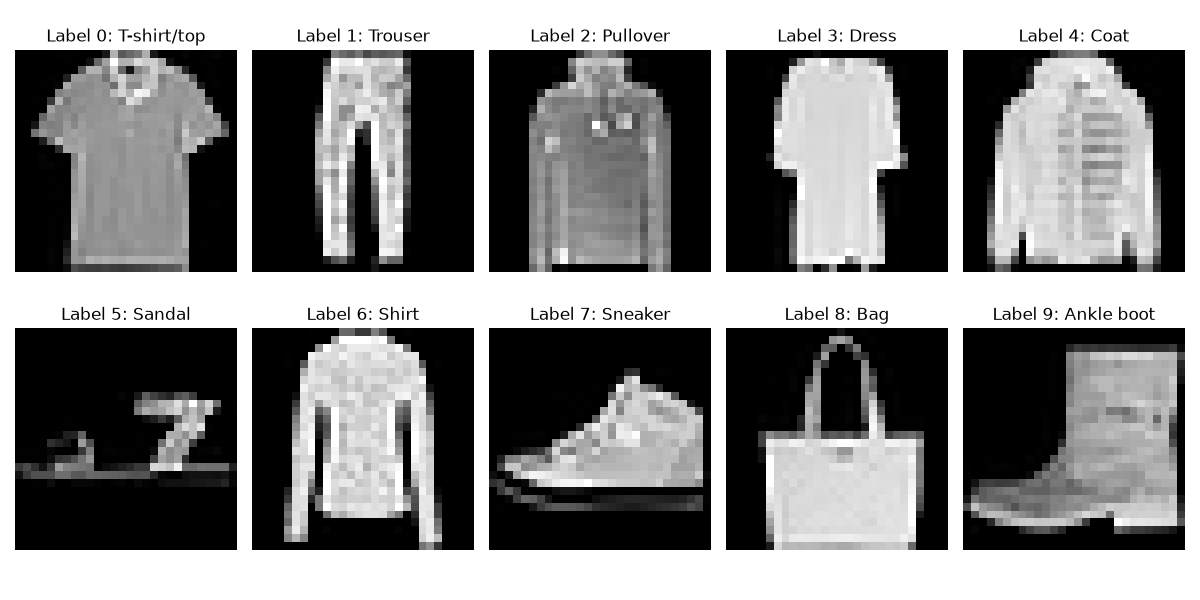
\includegraphics[width=\linewidth]{images/sample_images.png}
\caption{One representative training image per class, taken from the stored EDA output.}
\label{fig:samples}
\end{figure}
\FloatBarrier

\subsection{Data Splitting and Leakage Prevention}
\subsubsection{Official Test Set and Training--Validation Partitions}
The current pipeline leaves the official 10,000-image test set unchanged. Of the 60,000 official training images, a validation ratio of 0.15 reserves 9,000 for validation and leaves 51,000 for optimization. Table~\ref{tab:split} gives the protocol used by the current scripts; the earlier notebook uses a different partition, discussed separately in Section~\ref{sec:preliminary}.

\begin{table}[htbp]
\centering
\caption{Current data-splitting protocol.}
\label{tab:split}
\begin{tabular}{@{}lrl@{}}
\toprule
Partition & Images & Role \\
\midrule
Training & 51,000 & Parameter optimization \\
Validation & 9,000 & Checkpoint selection \\
Test & 10,000 & Final held-out evaluation \\
\bottomrule
\end{tabular}
\end{table}

\subsubsection{Split Sizes, Random Seed and Stratification Policy}
The split is generated with \texttt{random\_split} and a PyTorch generator seeded with 42. It operates at the image-index level and is \emph{not stratified}. The near-balanced training histogram is therefore an observed property of this seeded split, rather than an exact per-class allocation rule. The code applies no additional subset-selection rule beyond this train--validation division.

\subsubsection{Saved Split Indices, Subset Rules and Leakage Checks}
The split file stores training indices, validation indices, the seed, validation ratio and original dataset size. When reusing it, the loader checks metadata consistency, disjointness, duplicate indices, valid index ranges, expected partition sizes and complete coverage of the original training pool. Shared indices prevent different models from receiving different partitions.

These are checks on index membership. They do not constitute a search for visually duplicated images across the original benchmark files. Normalization is fitted only to training pixels, and model selection uses validation metrics instead of test metrics. Together, these choices reduce avoidable leakage through preprocessing and checkpoint selection.

\subsection{Preprocessing and Augmentation}
\subsubsection{Data Quality Checks, Tensor Conversion and Input Shapes}
The pipeline applies \texttt{ToImage}, scaled \texttt{float32} conversion and channel-wise normalization. It preserves the original resolution, with no resizing, padding or manual filtering. Labels remain integer class indices. Smoke checks cover shapes, types, finite values and label ranges; they are not a complete annotation audit.

\subsubsection{Normalization Using Training-Only Statistics}
For an original pixel value $u\in\{0,\ldots,255\}$, the transformed pixel is
\begin{equation}
 x=\frac{u/255-\mu_{\mathrm{train}}}{\sigma_{\mathrm{train}}}.
\end{equation}
Validation and test use the same training-derived statistics. Training records them in the resolved configuration; evaluation recomputes them from the saved split and verifies agreement within $10^{-6}$.

\subsubsection{Training Augmentation and Evaluation Transforms}
Optional \texttt{RandomAffine} rotation of $10^{\circ}$ precedes conversion and normalization. Augmentation is disabled in the current Linear, MLP and CNN configurations. Validation and test always omit stochastic augmentation. Future augmentation comparisons must identify the changed factor.

\subsubsection{Example Batch After Preprocessing}
Table~\ref{tab:batch} gives the interface derived from the code, not a new run. With batch size 128, the 51,000 training images produce 398 full batches and a final batch of 56; loss aggregation weights batches by sample count. A captured batch visualization from the final run is \textbf{TBD}.

\begingroup
\setlength{\intextsep}{6pt}
\begin{table}[!htbp]
\centering
\captionsetup{skip=6pt}
\caption{Expected full-batch interface under the current configuration.}
\label{tab:batch}
\begin{tabular}{@{}lll@{}}
\toprule
Tensor & Shape & Data type \\
\midrule
Images & $128\times1\times28\times28$ & \texttt{float32} \\
Labels & $128$ & \texttt{int64} \\
Model logits & $128\times10$ & Floating point \\
\bottomrule
\end{tabular}
\end{table}
\endgroup
